% Source for the figure of HugePageAllocator (sec. 5.9): a request of
% b = 5 MB, aligned to a huge page of 2 MB and rounded up to r = 6 MB, whose
% last MB of address space is never touched; given back, the block is kept
% by its thread for the next request of 6 MB only if r >= 8 MB, and so it
% goes back to the system. Build: make figures (in ../build).
\documentclass[border=4pt]{standalone}
\usepackage[T1]{fontenc}
\usepackage{newpxtext,newpxmath}
\usepackage[varqu,varl,scaled=0.95]{zi4}
\usepackage{tikz}
% tikz-ads.tex: the TikZ styles shared by the figures of the memory of the
% manual, \input by each standalone figure: a cell of a vector (cell), the
% cell that an operation touches (touched), a free cell (free), a node of a
% linked structure (node), the labels of indices (index) and of variables
% (var), a pointer (ptr), and \cells and \indices to draw a row of cells.
\usetikzlibrary{arrows.meta,positioning,calc,fit,shapes.multipart}
\definecolor{adsTouched}{RGB}{214,196,236}
\definecolor{adsFree}{RGB}{236,236,236}
\tikzset{
  ads/.style={>={Stealth[length=2mm]},font=\small,
              every node/.append style={inner sep=0pt}},
  cell/.style={draw,minimum width=7mm,minimum height=7mm,
               font=\small\ttfamily,outer sep=0pt},
  touched/.style={cell,fill=adsTouched},
  free/.style={cell,fill=adsFree,text=black!45},
  node/.style={draw,rounded corners=1pt,minimum width=8mm,
               minimum height=6mm,font=\small\ttfamily},
  index/.style={font=\scriptsize\ttfamily,text=black!60},
  var/.style={font=\small\itshape},
  ptr/.style={->,thick}
}
% \cells{name}{x,y}{list}: a row of cells, the first at (x,y), named
% name-0, name-1, ...; each item is text/style, the style one of cell,
% touched and free (e.g., {a/cell,e/touched,/free})
\newcommand{\cells}[3]{%
  \foreach \v/\s [count=\i from 0] in {#3}
    \node[\s] (#1-\i) at ($(#2)+(\i*7mm,0)$) {\v};}
% \indices{name}{n}: the indices 0 .. n-1 under the cells of name
\newcommand{\indices}[2]{%
  \foreach \i in {0,...,\numexpr#2-1\relax}
    \node[index,below=1.2mm of #1-\i] {\i};}

\usetikzlibrary{decorations.pathreplacing}
\begin{document}
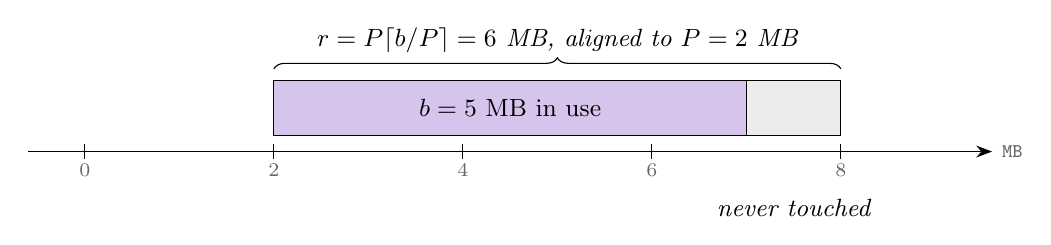
\begin{tikzpicture}[ads,x=12mm]
  % the address space, 2 MB a tick
  \draw[->] (-0.6,0) -- (9.6,0);
  \foreach \i in {0,2,...,8}
    \draw (\i,-1mm) -- (\i,1mm);
  \foreach \i/\t in {0/$0$,2/$2$,4/$4$,6/$6$,8/$8$}
    \node[index,below=1.5mm] at (\i,0) {\t};
  \node[index,anchor=west] at (9.7,0) {MB};
  % the block
  \node[touched,font=\small,minimum width=5*12mm,minimum height=7mm,anchor=south west]
    at (2,2mm) {$b = 5$ MB in use};
  \node[free,minimum width=12mm,minimum height=7mm,anchor=south west]
    at (7,2mm) {};
  \draw[decorate,decoration={brace,amplitude=4pt}]
    (2,10.5mm) -- (8,10.5mm) node[midway,above=2mm,var]
    {$r = P \lceil b / P \rceil = 6$ MB, aligned to $P = 2$ MB};
  \node[var,anchor=north] at (7.5,-6mm) {never touched};
\end{tikzpicture}
\end{document}
